
\chapter{\'AREA DE APLICACI\'ON}
\newpage
\section{Introducci\'on}

El presente proyecto propone una soluci\'on a un problema que se presenta con bastante frecuencia a la hora de crear y administrar el contenido de los sitios web creados con CMS's, Sistemas de Gesti\'on de Contenidos por su sigla en ingl\'es.\\
Con el desarrollo de un Sistema de Gesti\'on de Contenidos que pretende:

\begin{itemize}
\item Mejorar en tiempo.
\item Reducir las configuraciones necesarias para crear contenidos.
\item Crear un panel de administraci\'on interactivo e intuitivo.
\item Hacer gr\'afica la manera de manipular el contenido.
\item Facilitar la modificaci\'on de las plantillas en tiempo de ejecuci\'on.
\end{itemize}

La esencia del sistema se encuentra en lo intuitivo y la flexibilidad que ofrece en la gesti\'on del contenido, lo cual pretende mejorar la creaci\'on de contenidos y sobre todo facilitar la manipulaci\'on de los mismos, ya sea desde la administraci\'on avanzada o sobre las plantillas mismas.\\
El sistema es un CMS (Sistema de Gesti\'on de Contenidos) orientado principalmente a la creaci\'on de sitios Web.

\section{Antecedentes}
La administraci\'on de los sitios web siempre ha sido compleja debido a la forma de trabajo de las herramientas de administraci\'on, ya sea desde la misma actualizaci\'on de los contenidos que presenta, hasta la codificaci\'on de extensiones, por tal raz\'on surgieron los CMS (Sistemas de Gesti\'on de Contenidos) cuya principal tarea es  \textit{"Facilitar la creaci\'on, gesti\'on, distribuci\'on y publicaci\'on de informaci\'on"}.\\
Esta tarea se ha facilitado bastante gracias a los CMS's, pero muchas veces la poca experiencia sobre c\'omo administrarlos hace que la tarea de crear sitios siga siendo tediosa, otra situaci\'on que dificulta tambi\'en la creaci\'on y administraci\'on de sitios con CMS es que se tienen interfaces gr\'aficas poco amistosas y sobre todo poco intuitivas.
\newpage
\section{Identificaci\'on del problema}
\begin{figure}[h]
\centering
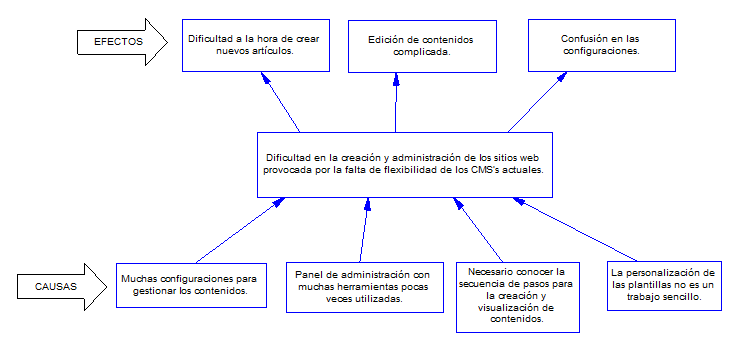
\includegraphics[scale=.75, keepaspectratio=true]{imagenes/01_imagen.png}
\caption{Arbol de problema}
\end{figure}

\section{Definici\'on del problema}
Una de las dificultades a la hora de crear y administrar sitios web dise\~nados con los CMS actuales es que muchas veces es necesario hacer varias configuraciones para poder gestionar (crear, editar, etc.) los contenidos.\\
A veces tenemos herramientas que vienen por defecto que muy pocas veces se utiliza, dando lugar a que el trabajo de administrar un sitio hecho con un CMS no sea intuitivo ni sencillo (Drupal, Zikula). Por otro lado esto tambi\'en provoca que tengamos un panel de administraci\'on bastante abarrotado.\\
Muchas veces es necesario conocer los pasos o la secuencia de creaci\'on de nuevos contenidos, y tambi\'en para mostrar los mismos.\\
En varios de los CMS's actuales la personalizaci\'on de las plantillas es un trabajo que requiere demasiado tiempo, adem\'as de que no es intuitivo.\\
Por lo tanto se define el problema como: \textit{Dificultad en la creaci\'on y administraci\'on de los sitios web provocada por la falta de flexibilidad de los CMS's actuales}.

\section{Innovaci\'on Tecnol\'ogica}
La creaci\'on de un CMS cuya principal caracter\'istica es ser gr\'afico y flexible, es un cambio que invierte de alguna manera la forma convencional de gestionar los contenidos permitiendo gestionar los contenidos de distintas maneras.

\section{Justificaci\'on}
Este proyecto facilitar\'a una herramienta que permitir\'a gestionar los contenidos, crearlos y posteriormente acomodarlo en las plantillas para su visualizaci\'on en los navegadores.\\
La herramienta resultante ser\'a de gran ayuda para todos los desarrolladores en menor o mayor medida, ya que no ser\'an necesarios tener grandes conocimientos acerca de CMS's para poder crear y administrar sitios web.\\
Muchas veces hemos o\'ido la frase ``El tiempo es oro'', pues bien, al reducir el tiempo de desarrollo de los sitios con el CMS resultante de este proyecto maximizamos la puesta en l\'inea de los sitios, facilit\'andole al cliente la posibilidad de trabajar con su sitio en muy poco tiempo.

\section{Alcances}
El proyecto no contempla de momento, la creaci\'on de extensiones para ampliar las funcionalidades del mismo pero si el soporte para las mismas.\\
Asimismo, entre las cosas que se contemplan en este proyecto cabe mencionar que este ser\'a un prototipo.\\
La herramienta resultante ser\'a capaz de facilitar:
\begin{itemize}
\item La creaci\'on de nuevos contenidos, como tambi\'en la edici\'on de los mismos.
\item La creaci\'on de nuevas secciones (Espacios donde se mostrar\'an los contenidos).
\item La gesti\'on de roles tales como Administrador, Editor y Visitante.
\item La manipulaci\'on de los contenidos y secciones de manera gr\'afica directamente sobre las plantillas.
\item La gesti\'on de contenidos secundarios.
\end{itemize}

\clearpage
